% === T05 - Orgasmall en Verilog ===
% David Alejandro Gonzalez Marquez
% fokerman@gmail.com
% https://github.com/fokerman/fpgaSoftcoreProgrammingCourse

\RequirePackage[2020-02-02]{latexrelease}

\documentclass[aspectratio=169]{beamer}
\usepackage{../packages}

\newcommand{\na}{\cellcolor{naranjauca}}
\newcommand{\gm}{\cellcolor{gray!50}} 

\title{\Huge Orgasmall en Verilog}
\author{David Alejandro González Márquez}
\institute{Programación de softcores en FPGAs\\
Programa de Profesoras/es Visitantes\\
Departamento de computación\\
Universidad de Buenos Aires}


\date{}

\lstset{
  backgroundcolor=\color{gray!20},   % choose the background color; you must add \usepackage{color} or \usepackage{xcolor}; should come as last argument
  basicstyle=\footnotesize,        % the size of the fonts that are used for the code
  breakatwhitespace=false,         % sets if automatic breaks should only happen at whitespace
  breaklines=true,                 % sets automatic line breaking
  extendedchars=true,              % lets you use non-ASCII characters; for 8-bits encodings only, does not work with UTF-8
  keepspaces=true,                 % keeps spaces in text, useful for keeping indentation of code (possibly needs columns=flexible)
  language=Verilog,                 % the language of the code
  showspaces=false,                % show spaces everywhere adding particular underscores; it overrides 'showstringspaces'
  showstringspaces=false,          % underline spaces within strings only
  showtabs=false,                  % show tabs within strings adding particular underscores
  tabsize=2,	                   % sets default tabsize to 2 spaces
  frame=single	                   % adds a frame around the code // topline bottomline leftline
}

\begin{document}

\begin{frame}[plain]
    \titlepage
    \begin{textblock}{110}(25,80)
    \begin{tcolorbox}[size=small,width=\textwidth,colback={gray!30},title={}]
    \begin{center}
     \scriptsize Clase disponible en: \url{https://github.com/fokerman/fpgaSoftcoreProgrammingCourse}
    \end{center}
    \end{tcolorbox}
    \end{textblock}
\end{frame}

\begin{frame}[fragile,t]
    \frametitle{Arquitectura \texttt{OrgaSmall}}
    \texttt{OrgaSmall} es un procesador (\emph{system on chip}) diseñado e implementado con fines didácticos.\\
    \textcolor{verdeuca}{Su implementación en \emph{Verilog} se denominada \textbf{\texttt{OrgaSmallSystem}}.}\\
    \begin{textblock}{110}(11,23)
    \only<2->{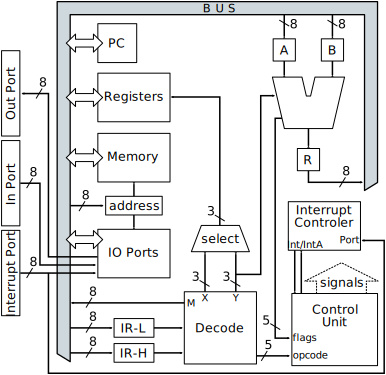
\includegraphics[scale=0.64]{img/arquitectura_micro_IO.pdf}}
    \end{textblock}
    \begin{textblock}{70}(80,23)
    \begin{itemize}
    \setlength\itemsep{0em}
    \item<2-> Arquitectura \emph{von Neumann}, memoria de datos e instrucciones compartida.
    \item<3-> 8 registros de propósito general, \texttt{R0} a \texttt{R7}.
    \item<3-> 1 registro de propósito específico PC.
    \item<4-> Tamaño de palabra de 8 bits e instrucciones de 16 bits.
    \item<4-> Memoria de 256 palabras de 8 bits.
    \item<5-> Bus de 8 bits.
    \item<5-> Diseño microprogramado.
    \item<6-> Soporta 3 puertos, 2 de entrada y 1 de salida mapeados a memoria.
    \item<6-> Una interrupción asociada a cambios sobre uno de los puertos de entrada.
    \end{itemize}
    \end{textblock}
\end{frame}

\begin{frame}[fragile,t]
    \frametitle{Arquitectura \texttt{OrgaSmall}\\ \small Codificación de instrucciones}
    \small
    Las instrucciones son de 16 bits en 4 posibles codificaciones.\\
    \textcolor{verdeuca}{Los primeros 5 bits indentifican el \texttt{opcode} de la instrucción, el resto de los bits indican sus parámetros.}
    \pause
    \begin{center}
    \begin{tabular}{c|l|l}
    Caso & Codificación               & Parámetros \\
    \hline
    A    & \texttt{\textcolor{r}{OOOOO} \textcolor{v}{XXX}\textcolor{verde}{YYY}\textcolor{gray}{-----}} & \texttt{\textcolor{v}{XXX}} = Registro X, \texttt{\textcolor{verde}{YYY}} = Registro Y o inmediato \\
    B    & \texttt{\textcolor{r}{OOOOO} \textcolor{v}{XXX}\textcolor{gray}{--------}} & \texttt{\textcolor{v}{XXX}} = Registro X\\
    C    & \texttt{\textcolor{r}{OOOOO} \textcolor{gray}{---}\textcolor{a}{MMMMMMMM}} & \texttt{\textcolor{a}{MMMMMMMM}} = Dirección de memoria o Inmediato\\
    D    & \texttt{\textcolor{r}{OOOOO} \textcolor{v}{XXX}\textcolor{a}{MMMMMMMM}}    & \texttt{\textcolor{v}{XXX}} = Registro X, \texttt{\textcolor{a}{MMMMMMMM}} = Dir. de memoria o Imm.\\
    \end{tabular}
    \end{center}
    \small
    \begin{itemize}
    \setlength\itemsep{0em}
    \item Los bits \texttt{\textcolor{v}{XXX}} codifican 8 registros posibles.
    \item Los bits \texttt{\textcolor{verde}{YYY}} codifican 8 registros posibles o un valor inmediato de 3 bits (\emph{shift}).
    \item Los bits \texttt{\textcolor{a}{MMMMMMMM}} codifican una dirección de memoria absoluta o un valor inmediato de 8 bits.
    \item Los valores indicados por \texttt{\textcolor{gray}{-}} deben valer cero.
    \end{itemize}
    Existen 32 opcodes posibles, 29 codifican instrucciones y 3 son reservados.\\
    \textcolor{gray}{Observación: En este diseño los opcode reservados dependen de la microarquitectura.}
    \normalsize
\end{frame}

\begin{frame}[fragile,t]
    \frametitle{Arquitectura \texttt{OrgaSmall}\\ \small Conjunto de instrucciones}
    \begin{textblock}{55}(5,19)
    \small
    \uncover<1->{
    \textbf{\texttt{Rx}} o \textbf{\texttt{Ry}}: Índices de registros,\\ número entre \texttt{0} y \texttt{7}.\\
    \vspace{0.2cm}
    \textbf{\texttt{M}}: Dirección de memoria o valor\\ inmediato, número de 8 bits.\\
    \vspace{0.2cm}
    \textbf{\texttt{t}}: Desplazamiento, número entre \texttt{0} y \texttt{7}.\\ Se codifica como \texttt{YYY} en 3 bits.\\
    }
    \bigskip
    \uncover<2->{
    Operador \textbf{\texttt{|}}: Identifica el registro usado como tope de la pila (ej. \texttt{|Rx|}).\\
    \vspace{0.2cm}
    \textbf{\texttt{|R7|}} es el registro de pila obligatorio para atender interrupciones.\\
    }
    \bigskip
    \uncover<3->{
    \textcolor{verdeuca}{La instrucción de \texttt{opcode} 15 es libre o reservada para futuras extensiones.}
    }
    \end{textblock}
    \begin{textblock}{100}(72,2)
    \tiny
    \begin{tabular}{l|l|l}
    Instrucción            & Acción                                                             & Codificación               \\
    \hline
    \texttt{Reservada}     & Codifica el \emph{Fetch} de instrucciones                          & \texttt{\textcolor{r}{00000}\textcolor{gray}{-----------}} \\  %00
    \texttt{ADD  Rx, Ry}   & \texttt{Rx} $\leftarrow$ \texttt{Rx + Ry}                          & \texttt{\textcolor{r}{00001}\textcolor{v}{XXX}\textcolor{verde}{YYY}\textcolor{gray}{-----}} \\  %01
    \texttt{ADC  Rx, Ry}   & \texttt{Rx} $\leftarrow$ \texttt{Rx + Ry + Flag\_C}                & \texttt{\textcolor{r}{00010}\textcolor{v}{XXX}\textcolor{verde}{YYY}\textcolor{gray}{-----}} \\  %02
    \texttt{SUB  Rx, Ry}   & \texttt{Rx} $\leftarrow$ \texttt{Rx - Ry}                          & \texttt{\textcolor{r}{00011}\textcolor{v}{XXX}\textcolor{verde}{YYY}\textcolor{gray}{-----}} \\  %03
    \texttt{AND  Rx, Ry}   & \texttt{Rx} $\leftarrow$ \texttt{Rx and Ry}                        & \texttt{\textcolor{r}{00100}\textcolor{v}{XXX}\textcolor{verde}{YYY}\textcolor{gray}{-----}} \\  %04
    \texttt{OR   Rx, Ry}   & \texttt{Rx} $\leftarrow$ \texttt{Rx or Ry}                         & \texttt{\textcolor{r}{00101}\textcolor{v}{XXX}\textcolor{verde}{YYY}\textcolor{gray}{-----}} \\  %05
    \texttt{XOR  Rx, Ry}   & \texttt{Rx} $\leftarrow$ \texttt{Rx xor Ry}                        & \texttt{\textcolor{r}{00110}\textcolor{v}{XXX}\textcolor{verde}{YYY}\textcolor{gray}{-----}} \\  %06
    \texttt{CMP  Rx, Ry}   & Modifica \texttt{flags} de \texttt{Rx - Ry}                        & \texttt{\textcolor{r}{00111}\textcolor{v}{XXX}\textcolor{verde}{YYY}\textcolor{gray}{-----}} \\  %07
    \texttt{MOV  Rx, Ry}   & \texttt{Rx} $\leftarrow$ \texttt{Ry}                               & \texttt{\textcolor{r}{01000}\textcolor{v}{XXX}\textcolor{verde}{YYY}\textcolor{gray}{-----}} \\  %08
    \hline
    \texttt{PUSH |Rx|, Ry} & \texttt{Mem[Rx]} $\leftarrow$ \texttt{Ry} ; \texttt{Rx} $\leftarrow$ \texttt{Rx-1}  & \texttt{\textcolor{r}{01001}\textcolor{v}{XXX}\textcolor{verde}{YYY}\textcolor{gray}{-----}} \\  %09
    \texttt{POP  |Rx|, Ry} & \texttt{Rx} $\leftarrow$ \texttt{Rx+1} ; \texttt{Ry} $\leftarrow$ \texttt{Mem[Rx]}  & \texttt{\textcolor{r}{01010}\textcolor{v}{XXX}\textcolor{verde}{YYY}\textcolor{gray}{-----}} \\  %10
    \texttt{CALL |Rx|, Ry} & \texttt{Mem[Rx]} $\leftarrow$ \texttt{PC} ; \texttt{Rx} $\leftarrow$ \texttt{Rx-1} ; \texttt{PC} $\leftarrow$ \texttt{Ry}  & \texttt{\textcolor{r}{01011}\textcolor{v}{XXX}\textcolor{verde}{YYY}\textcolor{gray}{-----}} \\  %11
    \texttt{CALL |Rx|, M}  & \texttt{Mem[Rx]} $\leftarrow$ \texttt{PC} ; \texttt{Rx} $\leftarrow$ \texttt{Rx-1} ; \texttt{PC} $\leftarrow$ \texttt{M}   & \texttt{\textcolor{r}{01100}\textcolor{v}{XXX}\textcolor{a}{MMMMMMMM}} \\  %12
    \texttt{RET  |Rx|}     & \texttt{Rx} $\leftarrow$ \texttt{Rx+1} ; \texttt{PC} $\leftarrow$ \texttt{Mem[Rx]}  & \texttt{\textcolor{r}{01101}\textcolor{v}{XXX}\textcolor{gray}{--------}} \\  %13
    \hline
    \texttt{RETI |Rx|}     & \texttt{Rx} $\leftarrow$ \texttt{Rx+1} ; \texttt{PC} $\leftarrow$ \texttt{Mem[Rx]} ;  & \texttt{\textcolor{r}{01110}\textcolor{v}{XXX}\textcolor{gray}{--------}} \\  %14
                           & \texttt{Rx} $\leftarrow$ \texttt{Rx+1} ; \texttt{Flags} $\leftarrow$ \texttt{Mem[Rx]} & \\
    \texttt{Libre}         &                                                                    & \texttt{\textcolor{r}{01111}\textcolor{gray}{-----------}} \\  %15
    \hline
    \texttt{STR  [M], Rx}  & \texttt{Mem[M]} $\leftarrow$ \texttt{Rx}                           & \texttt{\textcolor{r}{10000}\textcolor{v}{XXX}\textcolor{a}{MMMMMMMM}} \\  %16
    \texttt{LOAD Rx, [M]}  & \texttt{Rx} $\leftarrow$ \texttt{Mem[M]}                           & \texttt{\textcolor{r}{10001}\textcolor{v}{XXX}\textcolor{a}{MMMMMMMM}} \\  %17
    \texttt{STR  [Rx], Ry} & \texttt{Mem[Rx]} $\leftarrow$ \texttt{Ry}                          & \texttt{\textcolor{r}{10010}\textcolor{v}{XXX}\textcolor{verde}{YYY}\textcolor{gray}{-----}} \\  %18
    \texttt{LOAD Rx, [Ry]} & \texttt{Rx} $\leftarrow$ \texttt{Mem[Ry]}                          & \texttt{\textcolor{r}{10011}\textcolor{v}{XXX}\textcolor{verde}{YYY}\textcolor{gray}{-----}} \\  %19
    \hline
    \texttt{JMP M}         & \texttt{PC} $\leftarrow$ \texttt{M}                                & \texttt{\textcolor{r}{10100}\textcolor{gray}{---}\textcolor{a}{MMMMMMMM}} \\  %20
    \texttt{JC M}          & Si \texttt{flag\_C=1} entonces \texttt{PC} $\leftarrow$ \texttt{M} & \texttt{\textcolor{r}{10101}\textcolor{gray}{---}\textcolor{a}{MMMMMMMM}} \\  %21
    \texttt{JZ M}          & Si \texttt{flag\_Z=1} entonces \texttt{PC} $\leftarrow$ \texttt{M} & \texttt{\textcolor{r}{10110}\textcolor{gray}{---}\textcolor{a}{MMMMMMMM}} \\  %22
    \texttt{JN M}          & Si \texttt{flag\_N=1} entonces \texttt{PC} $\leftarrow$ \texttt{M} & \texttt{\textcolor{r}{10111}\textcolor{gray}{---}\textcolor{a}{MMMMMMMM}} \\  %23
    \texttt{JO M}          & Si \texttt{flag\_O=1} entonces \texttt{PC} $\leftarrow$ \texttt{M} & \texttt{\textcolor{r}{11000}\textcolor{gray}{---}\textcolor{a}{MMMMMMMM}} \\  %24
    \hline
    \texttt{SHRA Rx, t}    & \texttt{Rx} $\leftarrow$ \texttt{Rx} \verb|>>>| \texttt{t}         & \texttt{\textcolor{r}{11001}\textcolor{v}{XXX}\textcolor{verde}{YYY}\textcolor{gray}{-----}} \\  %25
    \texttt{SHR Rx, t}     & \texttt{Rx} $\leftarrow$ \texttt{Rx} \verb|>>| \texttt{t}          & \texttt{\textcolor{r}{11010}\textcolor{v}{XXX}\textcolor{verde}{YYY}\textcolor{gray}{-----}} \\  %26
    \texttt{SHL Rx, t}     & \texttt{Rx} $\leftarrow$ \texttt{Rx} \verb|<<| \texttt{t}          & \texttt{\textcolor{r}{11011}\textcolor{v}{XXX}\textcolor{verde}{YYY}\textcolor{gray}{-----}} \\  %27
    \hline
    \texttt{READF Rx}      & \texttt{Rx}    $\leftarrow$ \texttt{Flags}                         & \texttt{\textcolor{r}{11100}\textcolor{v}{XXX}\textcolor{gray}{--------}} \\  %28
    \texttt{LOADF Rx}      & \texttt{Flags} $\leftarrow$ \texttt{Rx}                            & \texttt{\textcolor{r}{11101}\textcolor{v}{XXX}\textcolor{gray}{--------}} \\  %29
    \hline
    \texttt{SET Rx, M}     & \texttt{Rx} $\leftarrow$ \texttt{M}                                & \texttt{\textcolor{r}{11110}\textcolor{v}{XXX}\textcolor{a}{MMMMMMMM}} \\  %30
    \hline
    \texttt{Reservada INT} & \texttt{Mem[R7]} $\leftarrow$ \texttt{Flags} ; \texttt{R7} $\leftarrow$ \texttt{R7-1} ; & \texttt{\textcolor{r}{11111}\textcolor{gray}{-----------}} \\  %31
                           & \texttt{Mem[R7]} $\leftarrow$ \texttt{PC} ; \texttt{R7} $\leftarrow$ \texttt{R7-1}      & \\
    \end{tabular}
    \end{textblock}
\end{frame}

\begin{frame}[fragile,t]
    \frametitle{Arquitectura \texttt{OrgaSmall}\\ \small Pila y Palabra de estado}
    \begin{textblock}{90}(17,22)
    
\includegraphics[scale=0.7]{img/mapa_de_memoria.pdf}
    \end{textblock}
    \begin{textblock}{90}(60,8)
    \uncover<1->{
    La pila está implementada \textbf{en memoria},\\ crece en el sentido de las \textbf{direcciones más bajas}.\\
    \textcolor{verdeuca}{El registro utilizado como tope de la pila,\\ apunta a la \textbf{primer dirección libre} en la pila.}\\
    }
    \bigskip
    \uncover<2->{
    Las intrucciones \texttt{PUSH}, \texttt{POP}, \texttt{CALL}, \texttt{RET} y \texttt{RETI} son las únicas que operan con la pila, \textbf{además de las interrupciones}.\\
    }
    \bigskip
%     Si bien es posible utilizar cualquier registro como pila, el mecanismo de interrupciones utiliza siempre el registro \texttt{R7} como pila.
    \uncover<3->{
    La palabra de estado es almacenada en la \texttt{ALU}, permitiendo ser modificada mediante dos operaciones específicas.\\
    }
    \bigskip
    \uncover<4->{
    \textcolor{verdeuca}{El orden de los bits de la palabra de estado es el siguiente:\\
    \textbf{\texttt{000I ONZC}} (desde más significativo a menos significativo).\\}
    \bigskip
    \textcolor{gray}{Donde \texttt{I} es el \emph{flag} de habilitación de interrupciones,\\ \texttt{O} (\emph{overflow}), \texttt{N} (\emph{negative}), \texttt{Z} (\emph{zero}) y \texttt{C} (\texttt{carry}).}
    }
    \end{textblock}
\end{frame}

\begin{frame}[fragile,t]
    \frametitle{Arquitectura \texttt{OrgaSmall}\\ \small Entrada-Salida e Interrupciones}
    \begin{textblock}{90}(17,22)
    
\includegraphics[scale=0.7]{img/mapa_de_memoria.pdf}
    \end{textblock}
    \begin{textblock}{90}(60,10)
    \noindent El sistema cuenta con 3 puertos de 8 bits:
    \begin{itemize}
    \setlength\itemsep{0em}
    \item<1-> \texttt{0xFC} : \small \textbf{\texttt{OutPort}} : Puerto de salida.
    \item<2-> \texttt{0xFD} : \small \textbf{\texttt{InPort}} : Puerto de entrada.
    \item<3-> \texttt{0xFE} : \small \textbf{\texttt{InterruptPort}} : Puerto de entrada sensible\\ \hspace{3.4cm} a interrupciones.
    \end{itemize}
    \vspace{0.2cm}
    \small
    \uncover<3->{
    Con el \emph{flag} de habilitación de interrupciones activado,\\
    el puerto \texttt{InterruptPort} \textcolor{naranjauca}{genera una interrupción} por cada \textbf{cambio de estado en alguno de sus bits}.\\
    }
    \bigskip
    \uncover<4->{
    \textcolor{naranjauca}{Detectada la interrupción}, el sistema carga en la pila los \emph{flags}, luego el \emph{PC} y por último se salta a la rutina de atención de interrupciones, tomando la dirección en \texttt{0xFF}.\\
    }
    \bigskip
    \uncover<5->{
    \textcolor{verdeuca}{Para todo este proceso, se utiliza como \emph{stack pointer} el registro \texttt{R7} que en el caso inicial se debe cargar en \texttt{0xFB}.}
    }
    \end{textblock}
\end{frame}


\begin{frame}[fragile,t]
    \frametitle{Procesador \texttt{OrgaSmall}: Componentes}
    \small
    Consiste en 8 componentes interconectados.
    \vspace{-0.2cm}
    \begin{center}
    \begin{tabular}{ll}
    \begin{minipage}{5cm}
    \begin{itemize}
    \footnotesize
    \setlength\itemsep{0cm}
    \item \texttt{Registers} (Banco de Registros)
    \item \texttt{PC} (Contador de Programa)
    \item \texttt{ALU} (Unidad Aritmético Lógica)
    \item \texttt{Memory} (Memoria)
    \end{itemize}
    \end{minipage}
    &
    \begin{minipage}{8cm}
    \begin{itemize}
    \footnotesize
    \setlength\itemsep{0cm}
    \item \texttt{IOports} (Puertos de Entrada/Salida)
    \item \texttt{Decode} (Decodificador de Instrucciones)
    \item \texttt{ControlUnit} (Unidad de Control)
    \item \texttt{InterruptControl} (Controlador de Interrupciones)
    \end{itemize}
    \end{minipage}
    \\
    \end{tabular}
    \end{center}
    \pause
    Cada uno de estos componentes es controlado desde la unidad de control por medio de las señales:
    \begin{center}
    \scriptsize
    \begin{tabular}[t]{llllllll}
    \texttt{\fbox{00}} & \texttt{RB\_enIn}           & \texttt{\fbox{08}} & \texttt{ALU\_enA}   & \texttt{\fbox{16}} & \texttt{JC\_microOp} & \texttt{\fbox{24}} & \texttt{DE\_enOutImm}   \\
    \texttt{\fbox{01}} & \texttt{RB\_enOut}          & \texttt{\fbox{09}} & \texttt{ALU\_enB}   & \texttt{\fbox{17}} & \texttt{JZ\_microOp} & \texttt{\fbox{25}} & \texttt{DE\_loadL}      \\
    \texttt{\fbox{02}} & \texttt{RB\_selectIndexIn}  & \texttt{\fbox{10}} & \texttt{ALU\_enOut} & \texttt{\fbox{18}} & \texttt{JN\_microOp} & \texttt{\fbox{26}} & \texttt{DE\_loadH}      \\
    \texttt{\fbox{03}} & \texttt{RB\_selectIndexOut} & \texttt{\fbox{11}} & \texttt{ALU\_opW}   & \texttt{\fbox{19}} & \texttt{JO\_microOp} & \texttt{\fbox{27}} & \texttt{INT\_ack}       \\
    \texttt{\fbox{04}} & \texttt{RB\_selectSP}       & \texttt{\fbox{12}} & \texttt{ALU\_OP$_0$}& \texttt{\fbox{20}} & \texttt{PC\_load}    & \texttt{\fbox{28}} & \texttt{-}              \\
    \texttt{\fbox{05}} & \texttt{MM\_enOut}          & \texttt{\fbox{13}} & \texttt{ALU\_OP$_1$}& \texttt{\fbox{21}} & \texttt{PC\_inc}     & \texttt{\fbox{29}} & \texttt{load\_Int\_microOp} \\
    \texttt{\fbox{06}} & \texttt{MM\_load}           & \texttt{\fbox{14}} & \texttt{ALU\_OP$_2$}& \texttt{\fbox{22}} & \texttt{PC\_enOut}   & \texttt{\fbox{30}} & \texttt{load\_microOp}  \\
    \texttt{\fbox{07}} & \texttt{MM\_enAddr}         & \texttt{\fbox{15}} & \texttt{ALU\_OP$_3$}& \texttt{\fbox{23}} & \texttt{-}           & \texttt{\fbox{31}} & \texttt{reset\_microOp} \\
    \end{tabular}
    \end{center}

\end{frame}

\begin{frame}[fragile,t]
    \frametitle{Procesador \texttt{OrgaSmall}: \texttt{modules}}
    \begin{textblock}{140}(10,10)
    El módulo del sistema se define como:
\lstset{basicstyle=\tiny}
\begin{lstlisting}
module OrgaSmallSystem(clk, reset, portOutput, portInput, portInterrupt);
\end{lstlisting}
    \begin{onlyenv}<2->
    El mismo está compuesto por los siguientes componentes:
\lstset{basicstyle=\tiny}
\begin{lstlisting}
module ArithmeticLogicUnit(clk, reset, A, B, O, enA, enB, enOut, OP, shift, flags, opW);
       ...
module Registers(clk, reset, inData, outData, enIn, enOut, selIn, selOut, setSP);
       ...
module ProgramCounter(clk, reset, inValue, outValue, PC_load, PC_inc, PC_enOut);
       ...
module Decode(clk, reset, halfInst, loadL, loadH, opcode, indexX, indexY, valueM);
       ...
module Memory(clk, reset, inData, outData, addr, enOut, load, enAddr, outAddr);
       ...
module IOports(clk, reset, inData, outData, load, addr, enOut, portOutput, portInput, portInterrupt);
       ...
module InterruptController(clk, reset, portInterrupt, intReq, intAck);
       ...
module ControlUnit(clk, reset, RB_enIn, RB_enOut, RB_selIndexIn, RB_selIndexOut, RB_setSP,
                   MM_enOut, MM_load, MM_enAddr, ALU_enA, ALU_enB, ALU_enOut, ALU_opW,
                   ALU_OP, PC_load, PC_inc, PC_enOut, DE_enOutImm, DE_loadL, DE_loadH,
                   ALU_flags, DE_opcode, IC_intReq, IC_intAck);
\end{lstlisting}
    \end{onlyenv}
    \begin{onlyenv}<3->
    A continuación vamos a estudiarlos uno a uno.
    \end{onlyenv}
    \end{textblock}
\end{frame}

\begin{frame}[fragile,t]
    \frametitle{Procesador \texttt{OrgaSmall}: \texttt{module ArithmeticLogicUnit}}
    \begin{textblock}{55}(10,10)
    \begin{onlyenv}<1->
\lstset{basicstyle=\tiny}
\begin{lstlisting}
module ArithmeticLogicUnit(clk, reset,
    A, B, O, enA, enB, enOut, OP,
    shift, flags, opW);
    input  clk, reset;
    input  [7:0] A, B;
    output [7:0] O;
    input  enA, enB, enOut;
    input  [3:0] OP;
    input  [2:0] shift;
    output [4:0] flags;
    input  opW;
    
    reg [8:0] qA, qB, qO;
    reg fI, fO, fN, fZ, fC;
    
    initial begin
        qA <= 0; qB <= 0; qO <= 0;
        fO <= 0; fN <= 0;
        fZ <= 0; fC <= 0;
        fI <= 0;
    end
    ...
\end{lstlisting}
\small
    Inicialización de todos los registros.\\
    Registros de \emph{flags} y de entrada y salida.\\
    \end{onlyenv}
    \end{textblock}
    \begin{textblock}{80}(70,10)
    \begin{onlyenv}<2->
\lstset{basicstyle=\tiny}
\begin{lstlisting}
 ...
 always @(posedge clk) begin
   case(OP)
     4'b0000 : begin  qO <= qO;                           end
     4'b0001 : begin  qO <= qA + qB;                      end
     4'b0010 : begin  qO <= qA + qB + {8'h0, fC};         end
     4'b0011 : begin  qO <= qA - qB;                      end
     4'b0100 : begin  qO <= qA & qB;                      end
     4'b0101 : begin  qO <= qA | qB;                      end 
     4'b0110 : begin  qO <= qA ^ qB;                      end 
     4'b0111 : begin  qO <= {qA[7],qA[7:0]} >>> shift;    end
     4'b1000 : begin  qO <= qA[7:0] >> shift;             end 
     4'b1001 : begin  qO <= qA[7:0] << shift;             end 
     4'b1010 : begin  qO <= {3'b000, fI, fO, fN, fZ, fC}; end
     4'b1100 : begin  qO <= 9'h000; end // cte 00
     4'b1101 : begin  qO <= 9'h001; end // cte 01
     4'b1110 : begin  qO <= 9'h002; end // cte 02
     4'b1111 : begin  qO <= 9'h0FF; end // cte ff
      default: begin  qO <= 9'h000; end
   endcase
 end
 ...
\end{lstlisting}
    \small
    Los resultados de las operaciones se generan en 9 bits.\\
    El cambio de \texttt{q0} es en \texttt{posedge} (flanco ascendente).\\
    \end{onlyenv}
    \end{textblock}
\end{frame}

\begin{frame}[fragile,t]
    \frametitle{Procesador \texttt{OrgaSmall}: \texttt{module ArithmeticLogicUnit}}
    \begin{textblock}{75}(10,10)
\lstset{basicstyle=\tiny}
\begin{lstlisting}
always @(negedge clk) begin
  if(enA) qA <= {1'h0,A};
  if(enB) qB <= {1'h0,B};
  if(reset) begin
    qA <= 0;
    qB <= 0;
  end
  if(opW) begin
    fN <= qO[7];
    fZ <= (qO[7:0] == 8'h0)? 1:0;
    if (OP==4'b0001 | OP==4'b0010 | OP==4'b0011)
      begin
          fC <= qO[8];
          fO <= (qO[8:7]==2'b01 || qO[8:7]==2'b10)? 1:0;
      end
    else
      begin
          fC <= 0;
          fO <= 0;
      end
  end
  if(OP==4'b1011) begin
    fI <= qA[4]; 
    fO <= qA[3]; 
    fN <= qA[2]; 
    fZ <= qA[1]; 
    fC <= qA[0];
  end
end
\end{lstlisting}
    \end{textblock}
    \begin{textblock}{60}(90,10)
    \begin{onlyenv}<2->
\lstset{basicstyle=\tiny}
\begin{lstlisting}
    ...

    assign flags = {fI, fO, fN, fZ, fC};
    assign O = enOut? qO[7:0] : 'bz;

endmodule
\end{lstlisting}
    \small
    En flanco descendente se actualizan todos los estados de:\\
    \begin{itemize}
    \item Registros de entrada \texttt{qA} y \texttt{qB}, dependiendo de las señales \texttt{enable}.
    \item Los \emph{flags} \texttt{fO}, \texttt{fN}, \texttt{fZ} y \texttt{fC} dependiendo del estado de la operación.
    \item Si la operación es 4, entonces se setean todos los \emph{flags}.
    \end{itemize}
    \end{onlyenv}
    \end{textblock}
\end{frame}

\begin{frame}[fragile,t]
    \frametitle{Procesador \texttt{OrgaSmall}: \texttt{module ArithmeticLogicUnit}}
    \begin{textblock}{80}(9,10)
    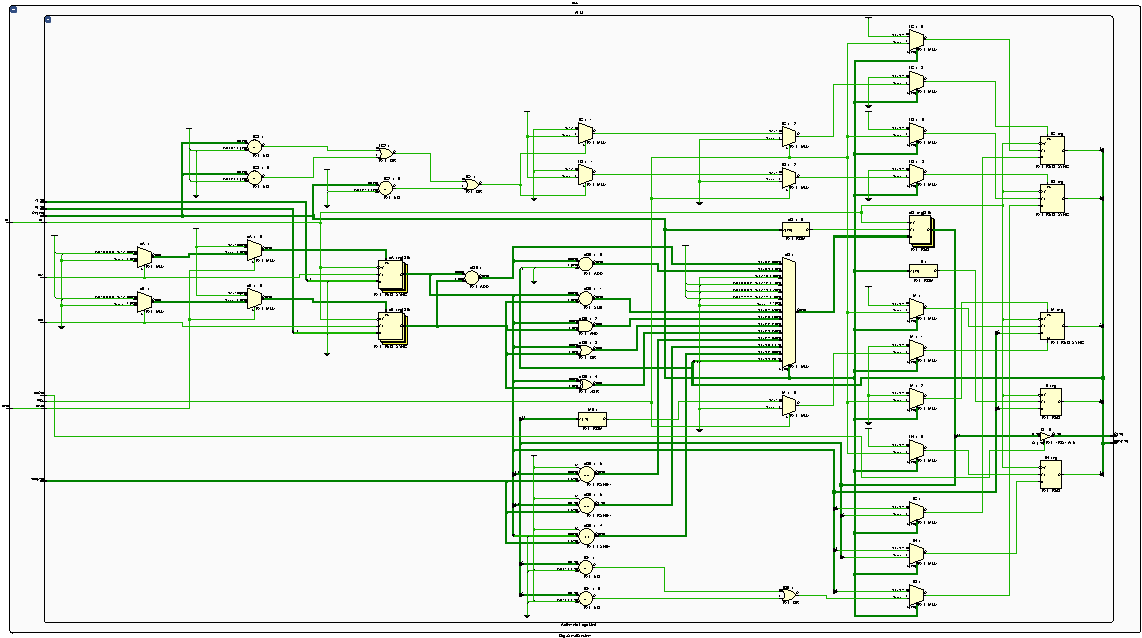
\includegraphics[scale=0.73]{pdf/schematicALU-crop.pdf}
    \end{textblock}
\end{frame}

\begin{frame}[fragile,t]
    \frametitle{Procesador \texttt{OrgaSmall}: \texttt{module ArithmeticLogicUnit}}
    \begin{textblock}{140}(10,7)
    \begin{center}
    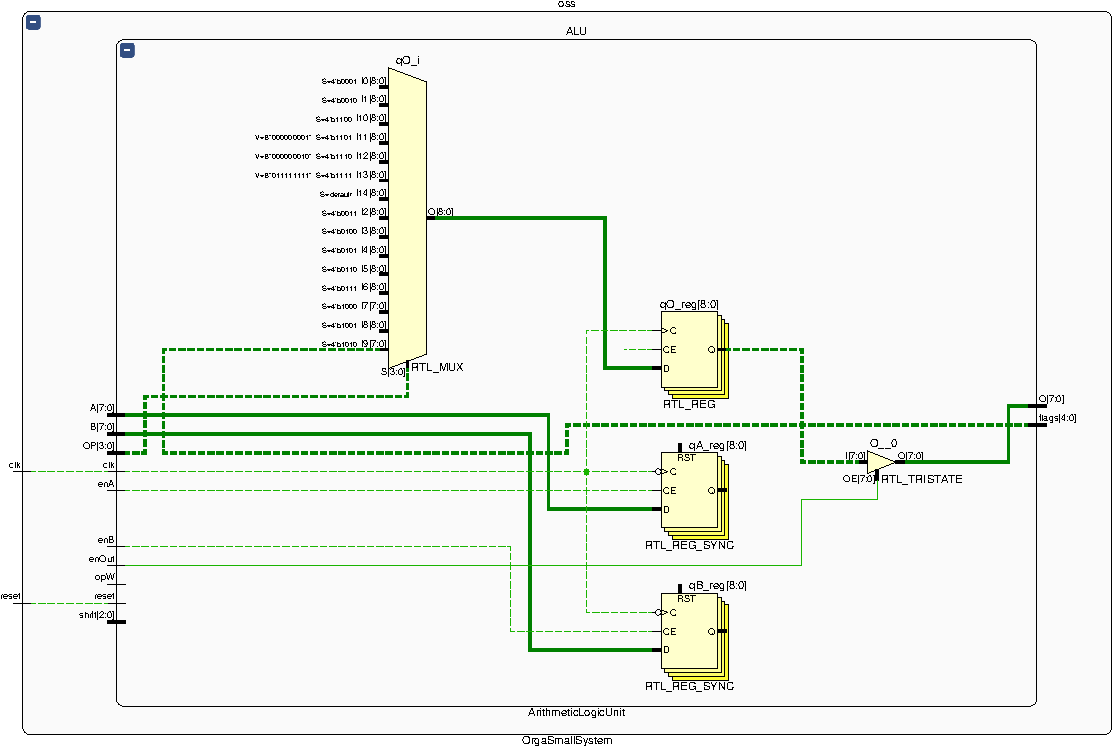
\includegraphics[scale=0.62]{pdf/schematicALU2-crop.pdf}
    \end{center}
    \end{textblock}
\end{frame}

\begin{frame}[fragile,t]
    \frametitle{Procesador \texttt{OrgaSmall}: \texttt{module Registers}}
    \begin{textblock}{80}(10,10)
\lstset{basicstyle=\tiny}
\begin{lstlisting}
module Registers(clk, reset, inData, outData,
                 enIn, enOut, selIn, selOut, setSP);
    input  clk, reset;
    input  [7:0] inData;
    output [7:0] outData;
    input  enIn, enOut;
    input [2:0] selIn, selOut;
    input setSP;
    
    reg [7:0] q [0:7];
    
    initial begin
        q[0] <= 0; q[1] <= 0; q[2] <= 0; q[3] <= 0;
        q[4] <= 0; q[5] <= 0; q[6] <= 0; q[7] <= 0;
    end
    always @(negedge clk) begin
        if(enIn) begin
            if(setSP)
                q[7] <= inData;
            else
                q[selIn] <= inData;
        end
        if(reset) begin
            q[0] <= 0; q[1] <= 0; q[2] <= 0; q[3] <= 0;
            q[4] <= 0; q[5] <= 0; q[6] <= 0; q[7] <= 0;
        end
    end
    assign outData = enOut? (setSP? q[7] : q[selOut]) : 'bz;
endmodule
\end{lstlisting}
    \end{textblock}
    \begin{textblock}{55}(95,12)
    \begin{onlyenv}<2->
    \small
    Los registros se declaran como un arreglo de registros, \texttt{q[0:7]} de tipo \texttt{reg [7:0]}\\
    \bigskip
    \textcolor{verdeuca}{Inicialmente se setean todos los registros a cero.}\\
    \end{onlyenv}
    \bigskip
    \begin{onlyenv}<3->
    La señal \texttt{setSP} sirve para setear el registro \texttt{r7}, usado como \emph{stack pointer}.\\
    \bigskip
    Si esta señal no está activa se utiliza \texttt{selIn} para seleccionar el registro a escribir.\\
    \bigskip
    \textcolor{verdeuca}{La salida utiliza también la señal \texttt{setSP} o \texttt{selOut} según corresponda.}
    \end{onlyenv}
    \end{textblock}
\end{frame}

\begin{frame}[fragile,t]
    \frametitle{Procesador \texttt{OrgaSmall}: \texttt{module Registers}}
    \begin{textblock}{140}(10,7)
    \begin{center}
    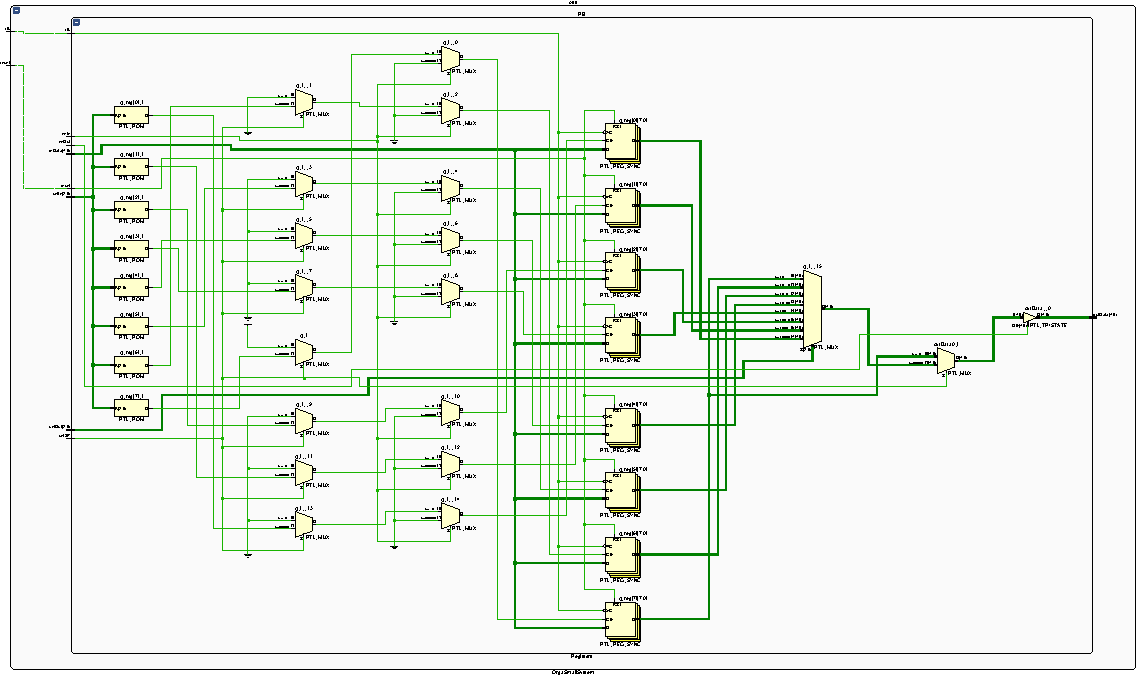
\includegraphics[scale=0.68]{pdf/schematicRB-crop.pdf}
    \end{center}
    \end{textblock}
\end{frame}

\begin{frame}[fragile,t]
    \frametitle{Procesador \texttt{OrgaSmall}: \texttt{module Registers}}
    \begin{textblock}{140}(10,7)
    \begin{center}
    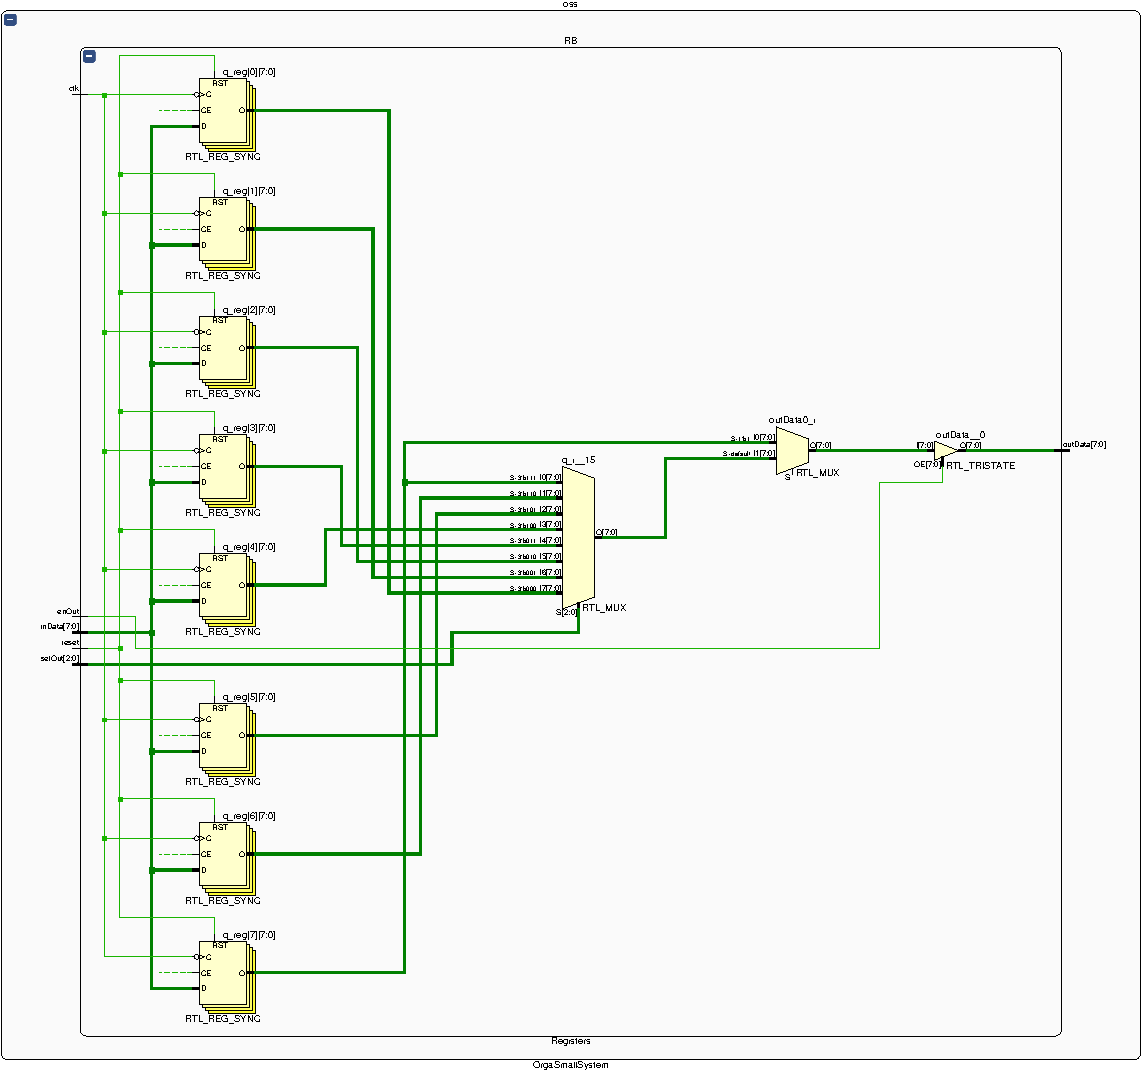
\includegraphics[scale=0.43]{pdf/schematicRB2-crop.pdf}
    \end{center}
    \end{textblock}
\end{frame}

\begin{frame}[fragile,t]
    \frametitle{Procesador \texttt{OrgaSmall}: \texttt{module ProgramCounter}}
    \begin{textblock}{70}(10,10)
\lstset{basicstyle=\tiny}
\begin{lstlisting}
module ProgramCounter(clk, reset, inValue, outValue,
                      PC_load, PC_inc, PC_enOut);

    input  clk, reset;
    input  [7:0] inValue;
    output [7:0] outValue;
    input  PC_load, PC_inc, PC_enOut;
    
    reg [7:0] q;
    
    initial begin
        q <= 'b0;
    end
    
    always @(negedge clk) begin
        if(reset)   q <= 'b0;
        if(PC_inc)  q <= q + 1;
        if(PC_load) q <= inValue;
    end
    
    assign outValue = PC_enOut? q : 'bz;
    
endmodule
\end{lstlisting}
    \end{textblock}
    \begin{textblock}{57}(90,12)
    \small
    \begin{onlyenv}<2->
    El \texttt{PC} es un registro declarado dentro del módulo como \texttt{q}.
    Su tamaño es de 8 bits.\\
    \bigskip
    \textcolor{verdeuca}{Inicialmente se setea el registro a cero.}\\
    \end{onlyenv}
    \bigskip
    \begin{onlyenv}<3->
    Tres señales modifican su estado:\\
    \begin{itemize}
    \setlength\itemsep{0cm}
     \item \texttt{reset}: Reset a cero.
     \item \texttt{PC\_inc}: Incrementar en 1.
     \item \texttt{PC\_load}: Cargar un valor arbitrario.
    \end{itemize}
    \bigskip
    La salida solo se expone en función del valor de \texttt{PC\_enOut}.
    \end{onlyenv}
    \end{textblock}
    \begin{textblock}{140}(10,74)
    \small
    \begin{onlyenv}<4->
    \textcolor{gray}{
    Este componente puede contener la lógica para incrementar de manera relativa el PC.\\
    Incluso debe prover el valor del PC para poder ser utilizado en calculo de direcciones.}
    \end{onlyenv}
    \end{textblock}
\end{frame}

\begin{frame}[fragile,t]
    \frametitle{Procesador \texttt{OrgaSmall}: \texttt{module ProgramCounter}}
    \begin{textblock}{140}(3,15)
    \begin{center}
    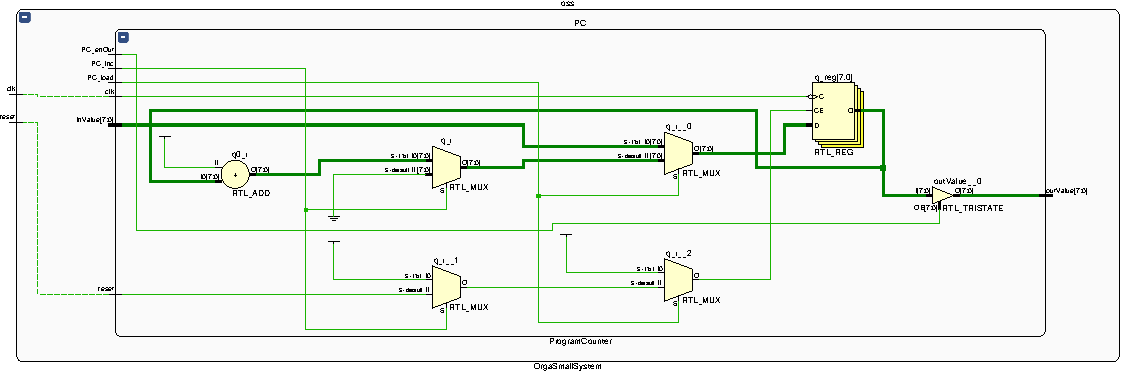
\includegraphics[scale=0.81]{pdf/schematicPC-crop.pdf}
    \end{center}
    \end{textblock}
\end{frame}

\begin{frame}[fragile,t]
    \frametitle{Procesador \texttt{OrgaSmall}: \texttt{module Decode}}
    \begin{textblock}{70}(10,10)
\lstset{basicstyle=\tiny}
\begin{lstlisting}
module Decode(clk, reset, halfInst, loadL, loadH,
              opcode, indexX, indexY, valueM);

    input  clk, reset;
    input [7:0] halfInst;
    input loadL, loadH;
    output [4:0] opcode;
    output [2:0] indexX, indexY;
    output [7:0] valueM;
    
    reg [15:0] q;
    
    initial begin
        q <= 'b0;
    end
    
    always @(negedge clk) begin
        if(loadL) q[7:0]  <= halfInst;
        if(loadH) q[15:8] <= halfInst;
        if(reset) q       <= 'b0;
    end

    //[15 14 13 12 11] [10 9 8] [7 6 5] [4 3 2 1 0]
    assign opcode = q[15:11];
    assign indexX = q[10:8];
    assign indexY = q[7:5];
    assign valueM = q[7:0];
    
endmodule
\end{lstlisting}
    \end{textblock}
    \begin{textblock}{55}(90,12)
    \small
    \begin{onlyenv}<2->
    La decodificación debe tomar \textbf{dos datos de memoria} para armar una instrucción.\\
    \bigskip
    Se utiliza un solo registro de 16 bits que \textbf{se carga parcialmente}.\\
    \end{onlyenv}
    \bigskip
    \begin{onlyenv}<3->
    La decodificación consiste tan solo en tomar los bits de la instrucción según el \textbf{formato de instrucción}.\\
    \bigskip
    \textcolor{verdeuca}{Notar que \texttt{valueM} se pisa con \texttt{indexY}.}\\
    \end{onlyenv}
    \bigskip
    \begin{onlyenv}<4->
    \textcolor{gray}{
    En otros casos, se puede requerir que algunos campos se generen de forma condicional. Agregando lógica combinatoria en la decodificación.}
    \end{onlyenv}
    \end{textblock}
\end{frame}

\begin{frame}[fragile,t]
    \frametitle{Procesador \texttt{OrgaSmall}: \texttt{module Decode}}
    \begin{textblock}{140}(8,15)
    \begin{center}
    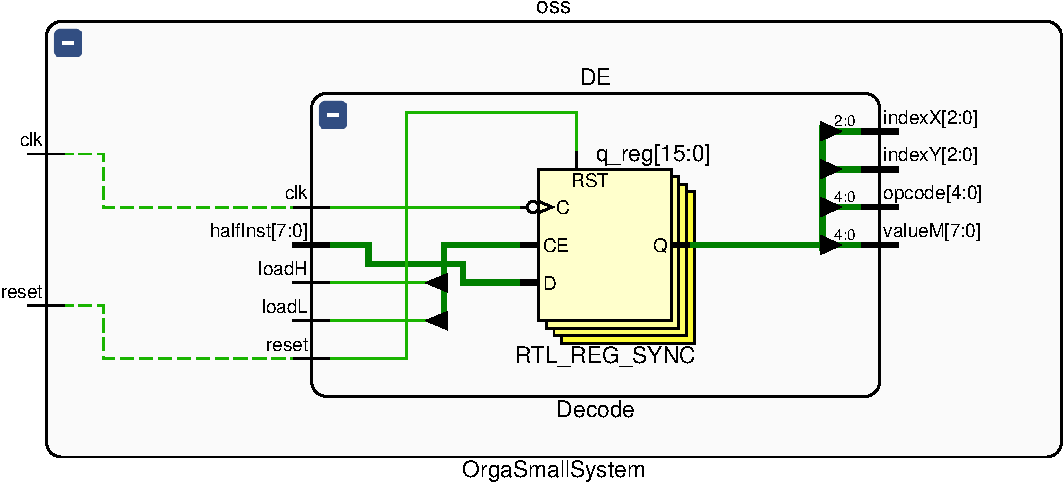
\includegraphics[scale=0.74]{pdf/schematicDE-crop.pdf}
    \end{center}
    \end{textblock}
\end{frame}

\begin{frame}[fragile,t]
    \frametitle{Procesador \texttt{OrgaSmall}: \texttt{module Memory}}
    \begin{textblock}{83}(10,10)
\lstset{basicstyle=\tiny}
\begin{lstlisting}
module Memory(clk, reset, inData, outData, addr,
              enOut, load, enAddr, outAddr);
    input  clk, reset;
    input  [7:0] inData;
    output [7:0] outData;
    input  [7:0] addr;
    input  enOut, load, enAddr;
    output [7:0] outAddr;
    
    reg [7:0] mem_addr;
    reg [7:0] mem [0:255];
    
    initial begin
        mem_addr <= 'b0;
        $readmemh("test00Verilog.mem", mem); 
    end
    
    always @(negedge clk) begin
        if(load & (mem_addr!=8'hfc & mem_addr!=8'hfd 
           & mem_addr!=8'hfe)) mem[mem_addr] <= inData;
        if(enAddr) mem_addr <= addr;
        if(reset)  mem_addr <= 'b0;
    end
    
    assign outData = (enOut & (mem_addr!=8'hfc & mem_addr!=8'hfd 
                      & mem_addr!=8'hfe))? mem[mem_addr] : 'bz;
    assign outAddr = mem_addr;
    
endmodule
\end{lstlisting}
    \end{textblock}
    \begin{textblock}{50}(100,12)
    \small
    \begin{onlyenv}<2->
    La memoria se declara como un \textbf{arreglo de 256 registros de 8 bits.}\\ \texttt{reg [7:0] mem[0:255]}\\
    \bigskip
    \textcolor{verdeuca}{La inicialización de la memoria se carga de un archivo utilizando la primitiva \texttt{\$readmemh}.}\\
    \end{onlyenv}
    \bigskip
    \begin{onlyenv}<3->
    Tiene además un registro de dirección que se \textbf{expone al exterior} del modulo mediante \texttt{outAddr}.\\
    \bigskip
    La memoria solo se lee o escribe para direcciones que \textbf{no estén mapeadas a entrada/salida}.
    \end{onlyenv}
    \end{textblock}
\end{frame}

\begin{frame}[fragile,t]
    \frametitle{Procesador \texttt{OrgaSmall}: \texttt{module Memory}}
    \begin{textblock}{140}(2,17)
    \begin{center}
    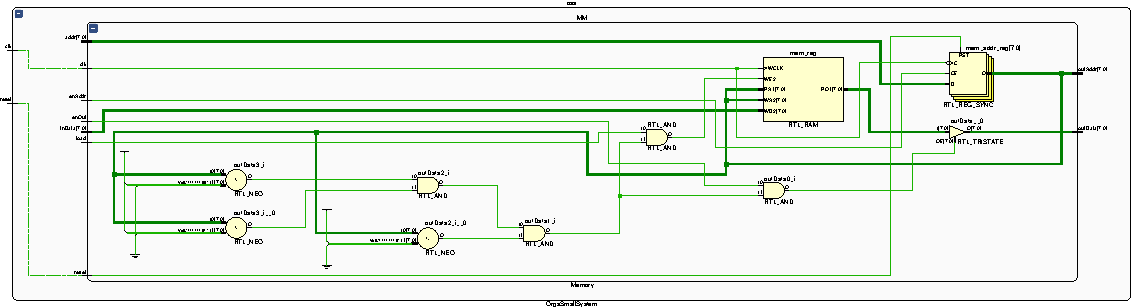
\includegraphics[scale=0.81]{pdf/schematicMM-crop.pdf}
    \end{center}
    \end{textblock}
\end{frame}

\begin{frame}[fragile,t]
    \frametitle{Procesador \texttt{OrgaSmall}: \texttt{module Memory}}
    \begin{textblock}{140}(10,15)
    \begin{center}
    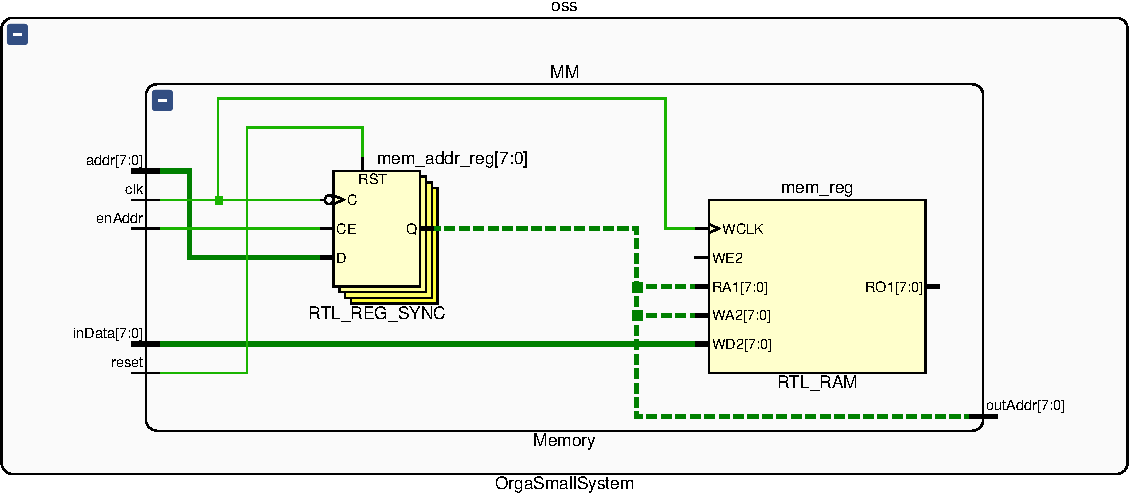
\includegraphics[scale=0.74]{pdf/schematicMM2-crop.pdf}
    \end{center}
    \end{textblock}
\end{frame}

\begin{frame}[fragile,t]
    \frametitle{Procesador \texttt{OrgaSmall}: \texttt{module IOports}}
    \begin{textblock}{58}(10,10)
    \begin{onlyenv}<1->
\lstset{basicstyle=\tiny}
\begin{lstlisting}
module IOports(clk, reset, inData, outData, 
               load, addr, enOut, portOutput,
               portInput, portInterrupt);
    input  clk, reset;
    input  [7:0] inData;
    output [7:0] outData;
    input  load;
    input  [7:0] addr;
    input  enOut;
    output [7:0] portOutput;
    input  [7:0] portInput;
    input  [7:0] portInterrupt;
    
    reg [7:0] qPOutput;
    reg [7:0] qPInput;
    reg [7:0] qPInterrupt;
    
    initial begin
        qPortOutput <= 8'h00;
        qPortInput <= 8'h00;
        qPortInterrupt <= 8'h00;   
    end
    ...
\end{lstlisting}
    \small
    Sean puertos de entrada o salida, todos están declarados como \textbf{registros}.
    \end{onlyenv}
    \end{textblock}
    \begin{textblock}{78}(73,10)
    \begin{onlyenv}<2->
\lstset{basicstyle=\tiny}
\begin{lstlisting}
    ...
    always @(negedge clk) begin
        if(addr==8'hfc && load)
            qPOutput <= inData;
        qPInput <= portInput;
        qPInterrupt <= portInterrupt;
        
        if(reset) begin
            qPOutput <= 8'hFF;
            qPInput <= 8'hFF;
            qPInterrupt <= 8'hFF;
        end
    end

    assign outData = (enOut & addr==8'hfc)? qPOutput   :'bz;
    assign outData = (enOut & addr==8'hfd)? qPInput    :'bz;
    assign outData = (enOut & addr==8'hfe)? qPInterrupt:'bz;
    assign portOutput = qPOutput;
    
endmodule
\end{lstlisting}
    \small
    El puerto de salida es el único que se escribe por una señal.\\
    El resto se \textbf{muestrean} sincrónicamente en cada \emph{clock}.\\
    \end{onlyenv}
    \begin{onlyenv}<3->
    \textcolor{verdeuca}{La salida se expone si \texttt{addr} tiene el valor correspondiente a la dirección mapeada del puerto.}
    \end{onlyenv}
    \end{textblock}
\end{frame}

\begin{frame}[fragile,t]
    \frametitle{Procesador \texttt{OrgaSmall}: \texttt{module IOports}}
    \begin{textblock}{140}(1,10)
    \begin{center}
    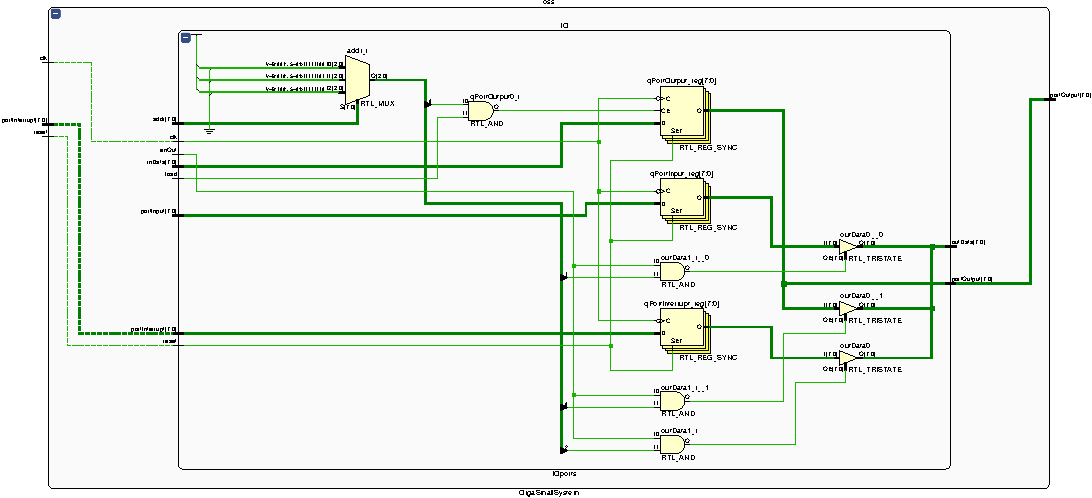
\includegraphics[scale=0.85]{pdf/schematicIO-crop.pdf}
    \end{center}
    \end{textblock}
\end{frame}

\begin{frame}[fragile,t]
    \frametitle{Procesador \texttt{OrgaSmall}: \texttt{module InterruptController}}
    \begin{textblock}{65}(10,10)
\lstset{basicstyle=\tiny}
\begin{lstlisting}
module InterruptController(clk, reset, 
                           portInterrupt, 
                           intReq, intAck);
    input  clk, reset;
    input  [7:0] portInterrupt;
    output intReq;
    input  intAck;
    
    reg [7:0] qnew;
    reg [7:0] q;
    reg interrupt;
    
    initial begin
        q <= 8'h00;
        qnew <= 8'h00;
        interrupt <= 0;        
    end
    ...
\end{lstlisting}
    \end{textblock}
    \begin{textblock}{65}(80,10)
    \begin{onlyenv}<2->
\lstset{basicstyle=\tiny}
\begin{lstlisting}
    ...
    always @(negedge clk) begin
        qnew <= portInterrupt;
        if(qnew != q) begin
            q <= qnew;
            interrupt <= 1;
        end
        if(intAck) interrupt <= 0;
        if(reset) begin
            q <= 8'h00;
            qnew <= 8'h00;
            interrupt <= 0;
        end 
    end
    
    assign intReq = interrupt;

endmodule
\end{lstlisting}
    \end{onlyenv}
    \end{textblock}
    \begin{textblock}{138}(10,62)
    \small
    \begin{onlyenv}<1->
     El objetivo es reconocer si el puerto de interrupciones cambio su valor, entonces se levantará la señal de interrupciones.
     \end{onlyenv}
     \begin{onlyenv}<2->
     \textcolor{verdeuca}{Para esto se guarda el valor anterior y el actual, \textbf{y se los compara}.\\}
    \end{onlyenv}
     \bigskip
     \begin{onlyenv}<3->
     La señal de interrupción se \textbf{debe reiniciar} indicando que la interrupción fue atendida.\\
     \end{onlyenv}
    \end{textblock}
\end{frame}

\begin{frame}[fragile,t]
    \frametitle{Procesador \texttt{OrgaSmall}: \texttt{module InterruptController}}
    \begin{textblock}{140}(1,16)
    \begin{center}
    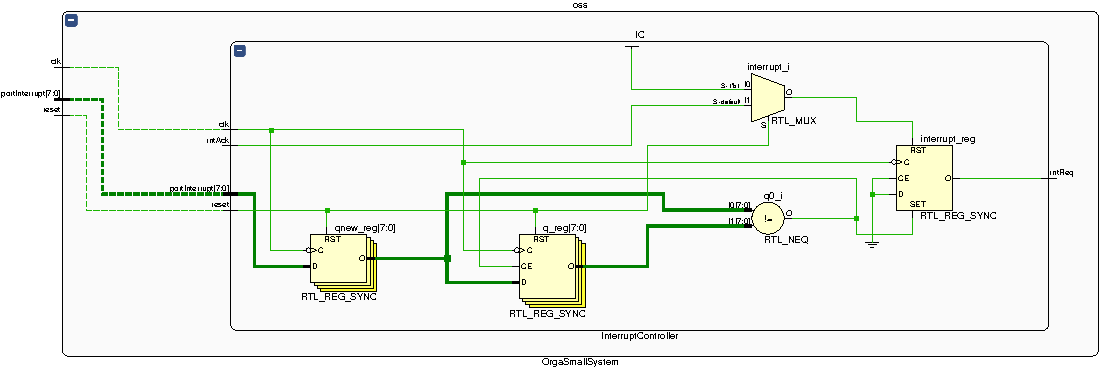
\includegraphics[scale=0.83]{pdf/schematicIC-crop.pdf}
    \end{center}
    \end{textblock}
\end{frame}

\begin{frame}[fragile,t]
    \frametitle{Procesador \texttt{OrgaSmall}: \texttt{module ControlUnit}}
    \begin{textblock}{90}(10,10)
\lstset{basicstyle=\tiny}
\begin{lstlisting}
module ControlUnit(clk, reset,
    RB_enIn, RB_enOut, RB_selIndexIn, RB_selIndexOut, RB_setSP,
    MM_enOut, MM_load, MM_enAddr,
    ALU_enA, ALU_enB, ALU_enOut, ALU_opW, ALU_OP, ALU_flags,
    PC_load, PC_inc, PC_enOut,
    DE_enOutImm, DE_loadL, DE_loadH, DE_opcode,
    IC_intReq, IC_intAck);

    input  clk, reset;
    output RB_enIn, RB_enOut, RB_selIndexIn, RB_selIndexOut, RB_setSP;
    output MM_enOut, MM_load, MM_enAddr;
    output ALU_enA, ALU_enB, ALU_enOut, ALU_opW;
    output [3:0] ALU_OP;
    output PC_load, PC_inc, PC_enOut;
    output DE_enOutImm, DE_loadL, DE_loadH;
    input  [4:0] ALU_flags;
    input  [4:0] DE_opcode;
    input  IC_intReq;
    output IC_intAck;
    
    wire JC_microOp, JZ_microOp, JN_microOp, JO_microOp;
    wire load_int_microOp, load_microOp, reset_microOp;
    reg [31:0] rom [0:511];
    reg [8:0] microOp = 0;

    initial begin
        $readmemh("microCodeVerilog.mem", rom); 
    end
    ...
\end{lstlisting}
    \end{textblock}
    \begin{textblock}{45}(105,12)
    \small
    \begin{onlyenv}<2->
    Este módulo contiene una gran memoria para estados.\\
    \bigskip
    \textcolor{verdeuca}{Por diseño se tienen 512 estados con 32 señales cada uno.
    Aunque la mayor parte no se utiliza.}\\
    \end{onlyenv}
    \bigskip
    \begin{onlyenv}<3->
    Los estados se carga inicialmente de un archivo que contiene el conjunto de microinstrucciones o señales, que programan la máquina Orgasmall.\\
    \bigskip
    \textcolor{verdeuca}{Alterando estas señales es posible contruir diferentes instrucciones.}
    \end{onlyenv}
    \end{textblock}
\end{frame}

\begin{frame}[fragile,t]
    \frametitle{Procesador \texttt{OrgaSmall}: \texttt{module ControlUnit}}
    \begin{textblock}{90}(10,10)
\lstset{basicstyle=\tiny}
\begin{lstlisting}
    ...
    always @(negedge clk) begin
        if(load_microOp & JC_microOp & ALU_flags[0])
           microOp <= microOp + 2;
        else
        if(load_microOp & JZ_microOp & ALU_flags[1])
            microOp <= microOp + 2;
        else
        if(load_microOp & JN_microOp & ALU_flags[2])
            microOp <= microOp + 2;
        else
        if(load_microOp & JO_microOp & ALU_flags[3])
            microOp <= microOp + 2;
        else
        if(load_microOp & load_int_microOp & ALU_flags[4] & IC_intReq)
            microOp <= 9'h1f0;
        else
        if(load_microOp & !JC_microOp & !JZ_microOp 
           & !JN_microOp & !JO_microOp & !load_int_microOp)
            microOp <= { DE_opcode, 4'b0000 };
        else
            microOp <= microOp + 1;
            
        if(reset | reset_microOp) microOp <= 0;
    end
    ...
\end{lstlisting}
    \end{textblock}
    \begin{textblock}{47}(105,12)
    \small
    El microPC o contador de estados, siempre se incrementa en 1.\\
    \bigskip
    \begin{onlyenv}<2->
    A excepción de tres situaciones.\\
    \begin{itemize}
     \item Operaciones de salto condicional.
     \item Salto a la rutina de interrupciones.
     \item Salto a la instrucción decodificada.
    \end{itemize}
    \end{onlyenv}
    \end{textblock}
\end{frame}

\begin{frame}[fragile,t]
    \frametitle{Procesador \texttt{OrgaSmall}: \texttt{module ControlUnit}}
    \begin{textblock}{65}(10,10)
    \begin{onlyenv}<1->
\lstset{basicstyle=\tiny}
\begin{lstlisting}
    ...
    assign RB_enIn        = rom[microOp][0];
    assign RB_enOut       = rom[microOp][1];
    assign RB_selIndexIn  = rom[microOp][2];
    assign RB_selIndexOut = rom[microOp][3];
    assign RB_setSP       = rom[microOp][4];
    
    assign MM_enOut       = rom[microOp][5];
    assign MM_load        = rom[microOp][6];
    assign MM_enAddr      = rom[microOp][7];
                      
    assign ALU_enA        = rom[microOp][8];
    assign ALU_enB        = rom[microOp][9];
    assign ALU_enOut      = rom[microOp][10];
    assign ALU_opW        = rom[microOp][11];
    
    assign ALU_OP         = { rom[microOp][15],
                              rom[microOp][14],
                              rom[microOp][13],
                              rom[microOp][12] };
    
    assign JC_microOp     = rom[microOp][16];
    assign JZ_microOp     = rom[microOp][17];
    assign JN_microOp     = rom[microOp][18];
    assign JO_microOp     = rom[microOp][19];
    ...
\end{lstlisting}
    \end{onlyenv}
    \end{textblock}
    \begin{textblock}{65}(80,10)
    \begin{onlyenv}<2->
\lstset{basicstyle=\tiny}
\begin{lstlisting}
    ...
    assign PC_load          = rom[microOp][20];
    assign PC_inc           = rom[microOp][21];
    assign PC_enOut         = rom[microOp][22];
                           // rom[microOp][23];
    
    assign DE_enOutImm      = rom[microOp][24];
    assign DE_loadL         = rom[microOp][25];
    assign DE_loadH         = rom[microOp][26];
    assign IC_intAck        = rom[microOp][27];
                           // rom[microOp][28];
    
    assign load_int_microOp = rom[microOp][29];
    assign load_microOp     = rom[microOp][30];
    assign reset_microOp    = rom[microOp][31];
    
endmodule
\end{lstlisting}
    \small
    Todas las señales leídas de la memoria son asignadas a cables o registros del circuito.\\
    \bigskip
    \textcolor{verdeuca}{Luego son utilizadas fuera y dentro del circuito.}
    \end{onlyenv}
    \end{textblock}
\end{frame}

\begin{frame}[fragile,t]
    \frametitle{Procesador \texttt{OrgaSmall}: \texttt{module ControlUnit}}
    \begin{textblock}{140}(1,16)
    \begin{center}
    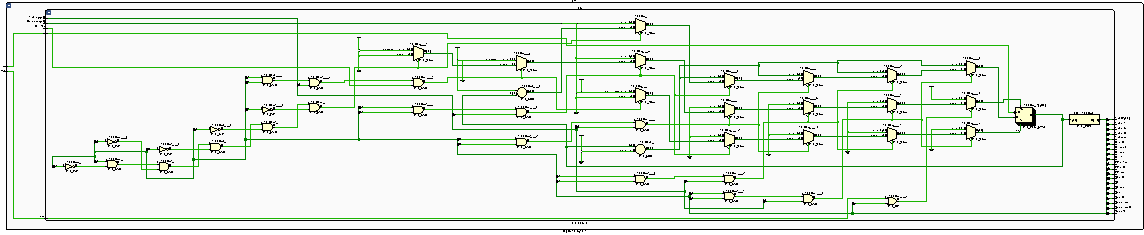
\includegraphics[scale=0.81]{pdf/schematicCU-crop.pdf}
    \end{center}
    \end{textblock}
\end{frame}

\begin{frame}[fragile,t]
    \frametitle{Procesador \texttt{OrgaSmall}: \texttt{module ControlUnit}}
    \begin{textblock}{140}(5,10)
    \begin{center}
    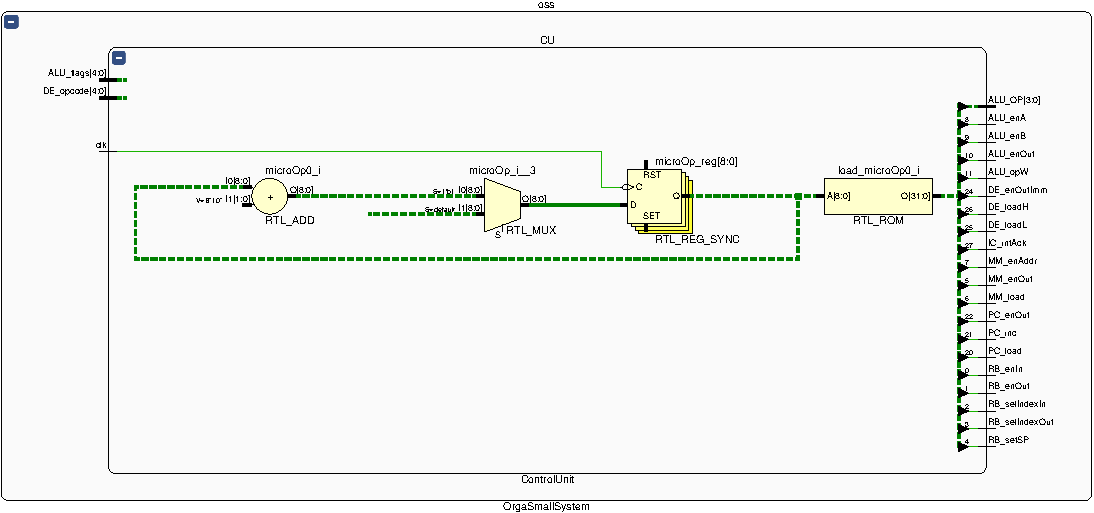
\includegraphics[scale=0.8]{pdf/schematicCU2-crop.pdf}
    \end{center}
    \end{textblock}
\end{frame}

\begin{frame}[fragile,t]
    \frametitle{Procesador \texttt{OrgaSmall}: \texttt{module OrgaSmallSystem}}
    \begin{textblock}{60}(10,10)
    \begin{onlyenv}<1->
\lstset{basicstyle=\tiny}
\begin{lstlisting}
module OrgaSmallSystem(clk, reset, portOutput,
                    portInput, portInterrupt);

    input clk, reset;
    
    output [7:0] portOutput;
    input  [7:0] portInput;
    input  [7:0] portInterrupt;
 
    wire [7:0] BUS;
    wire ALU_enA, ALU_enB, ALU_enOut, ALU_opW;
    wire [3:0] ALU_OP;
    wire [4:0] ALU_flags;
    wire RB_enIn, RB_enOut, RB_setSP;
    wire [2:0] RB_selIn, RB_selOut;
    wire PC_load, PC_inc, PC_enOut;
    wire DE_enOutImm, DE_loadL, DE_loadH;
    wire [4:0] DE_opcode;
    wire MM_enOut, MM_load, MM_enAddr;
    wire [2:0] DE_indexX, DE_indexY;
    wire [7:0] DE_valueM;
    wire [7:0] outAddr;
    wire IC_intReq, IC_intAck;
    wire RB_selIndexIn, RB_selIndexOut;
    ...
\end{lstlisting}
    \small
    Declaración de todos los cables requeridos.
    \end{onlyenv}
    \end{textblock}
    \begin{textblock}{72}(75,10)
    \begin{onlyenv}<2->
\lstset{basicstyle=\tiny}
\begin{lstlisting}
    ...
    ArithmeticLogicUnit ALU(clk, reset, BUS, BUS, BUS, 
      ALU_enA, ALU_enB, ALU_enOut, ALU_OP, DE_indexY,
      ALU_flags, ALU_opW);
    
    Registers RB(clk, reset, BUS, BUS, RB_enIn,
      RB_enOut, RB_selIn, RB_selOut, RB_setSP);
    
    ProgramCounter PC(clk, reset, BUS, BUS,
      PC_load, PC_inc, PC_enOut);
    
    Decode DE(clk, reset, BUS, DE_loadL, DE_loadH,
      DE_opcode, DE_indexX, DE_indexY, DE_valueM);
        
    Memory MM(clk, reset, BUS, BUS, BUS,
      MM_enOut, MM_load, MM_enAddr, outAddr);

    IOports IO(clk, reset, BUS, BUS, MM_load, outAddr,
      MM_enOut, portOutput, portInput, portInterrupt);
        
    InterruptController IC(clk, reset, portInterrupt,
      IC_intReq, IC_intAck);
    ...
\end{lstlisting}
    \small
    Se instancia uno a uno los componentes del \emph{datapath}.\\
    \end{onlyenv}
    \begin{onlyenv}<3->
    \small
    \textcolor{verdeuca}{Se respeta el orden de los parámetros,} \textcolor{rojo}{aunque se dificulta la lectura. \textbf{Ejemplo: señal \texttt{BUS} duplicada.}}
    \end{onlyenv}
    \end{textblock}
\end{frame}

\begin{frame}[fragile,t]
    \frametitle{Procesador \texttt{OrgaSmall}: \texttt{module OrgaSmallSystem}}
    \begin{textblock}{90}(10,10)
\lstset{basicstyle=\tiny}
\begin{lstlisting}
    ...
    ControlUnit CU(clk, reset,
        RB_enIn, RB_enOut, RB_selIndexIn, RB_selIndexOut, RB_setSP,
        MM_enOut, MM_load, MM_enAddr,
        ALU_enA, ALU_enB, ALU_enOut, ALU_opW, ALU_OP, ALU_flags,
        PC_load, PC_inc, PC_enOut,
        DE_enOutImm, DE_loadL, DE_loadH, DE_opcode,
        IC_intReq, IC_intAck);
    
    assign RB_selIn  = RB_selIndexIn?  DE_indexY : DE_indexX;
    assign RB_selOut = RB_selIndexOut? DE_indexY : DE_indexX;
    assign BUS       = DE_enOutImm?    DE_valueM : 'bz;
    
endmodule
\end{lstlisting}
    \end{textblock}
    \begin{textblock}{40}(105,12)
    \small
    \begin{onlyenv}<2->
    Por último se instancia la únidad de control.\\
    \bigskip
    \textcolor{verdeuca}{Donde se conecta el resto de las señales declaradas como cables.}
    \end{onlyenv}
    \end{textblock}
    \begin{textblock}{140}(10,52)
    \small
    \begin{onlyenv}<3->
    El \emph{datapath} se completa generando las señales desde el decodificador a la selección de registros en el\\
    banco de registros. \textcolor{verdeuca}{Se identifica como los dos multiplexores de selección de registros.}\\
    \end{onlyenv}
    \bigskip
    \begin{onlyenv}<4->
    Además generando la señal desde el decodificador al bus principal del valor \texttt{M}. \textcolor{verdeuca}{Leer el valor inmediato.}\\
    \end{onlyenv}
    \bigskip
    \begin{onlyenv}<5->
    \textcolor{gray}{Notar que estos elementos podian formar parte de los módulos, sin embargo se busco respetar el esquema del \emph{datapath}.}
    \end{onlyenv}
    \end{textblock}
\end{frame}

\begin{frame}[fragile,t]
    \frametitle{Procesador \texttt{OrgaSmall}: \texttt{module OrgaSmallSystem}}
    \begin{textblock}{140}(2,14)
    \begin{center}
    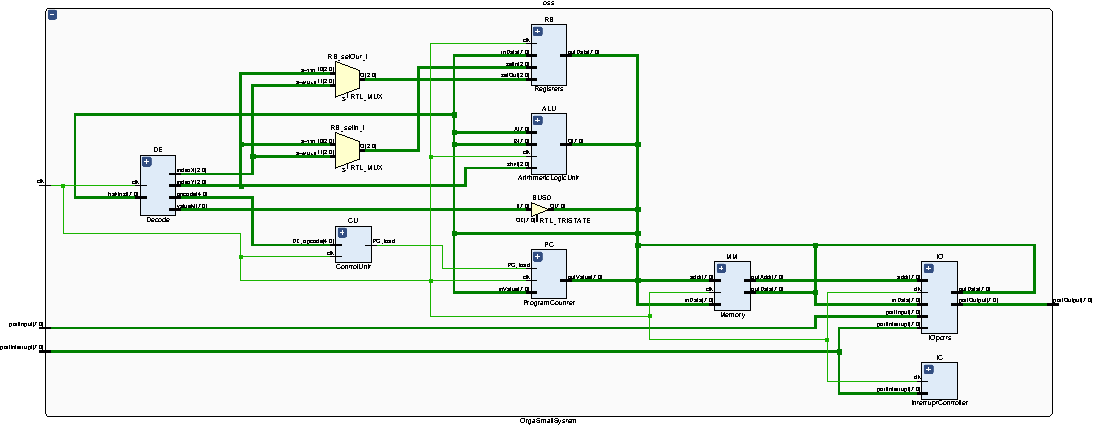
\includegraphics[scale=0.84]{pdf/schematic-crop.pdf}
    \end{center}
    \end{textblock}
\end{frame}

\begin{frame}[fragile,t]
    \frametitle{\texttt{Ejemplo Completo: Contador con salida serie}}
    \begin{textblock}{50}(10,10)
\lstset{basicstyle=\tiny,language={[x86masm]Assembler},morekeywords={SET, LOAD, LOADF}}
\begin{lstlisting}
SET R7, 0xFB  ; set STACK
SET R0, interrupt_handler
STR  [0xFF], R0 ; Set Interrupt Rutine
SET R0, 0x10
LOADF R0 ; Set Interrupt Flag

; main
SET R0, 0x0
SET R1, 0x1
whileTrue:
    STR [0xFC], R1 ; out <- 0001
    CALL |R7|, sleep
    STR [0xFC], R0 ; out <- 0000
    SET R3, 0x7
    whileSerie:
        CALL |R7|, sleep
        LOAD R2, [current]
        AND R2, R1
        SHL R2, 1
        STR [0xFC], R2 ; out <- 00X0
        LOAD R2, [current]
        SHR R2, 1
        STR [current], R2
        SUB R3, R1
        JZ continuar
        JMP whileSerie
    continuar:
    LOAD R2, [data]
    STR [current], R2
JMP whileTrue
\end{lstlisting}
    \end{textblock}
    \begin{textblock}{30}(70,10)
\lstset{basicstyle=\tiny,language={[x86masm]Assembler},morekeywords={SET, LOAD, LOADF}}
\begin{lstlisting}
sleep:
    PUSH |R7|, R0
    PUSH |R7|, R1
    PUSH |R7|, R2
    PUSH |R7|, R3
    PUSH |R7|, R4
    SET R2, 10
    ciclo:
        CMP R2, R0
        JZ end_sleep
        SUB R2, R1
        JMP ciclo
    end_sleep:
    POP  |R7|, R4
    POP  |R7|, R3
    POP  |R7|, R2
    POP  |R7|, R1
    POP  |R7|, R0
    RET  |R7|

current:  DB 0x00
data:     DB 0x00

; Memory
; 0x00 = entry point
; 0xFB = stack base
; 0xFC = port Output
; 0xFD = port Input
; 0xFE = port Interrupt
; 0xFF = Rutine pointer
\end{lstlisting}
    \end{textblock}
    \begin{textblock}{40}(110,10)
\lstset{basicstyle=\tiny,language={[x86masm]Assembler},morekeywords={SET, LOAD, LOADF}}
\begin{lstlisting}
interrupt_handler:
    PUSH |R7|, R0
    PUSH |R7|, R1
    PUSH |R7|, R2
    PUSH |R7|, R3
    PUSH |R7|, R4
    SET R0, 0x1
    SET R1, 0x2
    LOAD R3, [0xFE]
    CMP R3, R0
    JZ val_inc
    CMP R3, R1
    JZ val_dec
    end_interrupt:
    POP  |R7|, R4
    POP  |R7|, R3
    POP  |R7|, R2
    POP  |R7|, R1
    POP  |R7|, R0
    RETI |R7|
    val_inc:
        LOAD R3, [data]
        ADD R3, R0
        STR [data], R3
        JMP end_interrupt
    val_dec:
        LOAD R3, [data]
        SUB R3, R0
        STR [data], R3
        JMP end_interrupt
\end{lstlisting}
    \end{textblock}
\end{frame}

\begin{frame}[fragile]
    \frametitle{Observaciones \texttt{OrgaSmall}}
    La arquitectura del sistema como su microarquitectura están \textbf{diseñadas con fines didácticos}.\\
    \vspace{0.2cm}
    Su espacio de direccionamiento y tipos de direccionamiento son \textbf{muy limitados}.\\
    \vspace{0.2cm}
    No está pensado para soportar desplazamientos a memoria, todas \textbf{direcciones absolutas}.\\
    \vspace{0.2cm}
    \pause
    El diseño de las instrucciones es regular para simplificar \textbf{su lectura y decodificación.}\\
    \vspace{0.2cm}
    Soporta instrucciones complejas, ya que \textbf{no tiene seudoinstrucciones}.\\
    \vspace{0.2cm}
    El diseño de la microarquitectura tiene múltiples \textbf{registros innecesarios}.\\
    \vspace{0.2cm}
    \pause
    Es un diseño escalable y adaptable para \textbf{nuevas instrucciones}.\\
    \vspace{0.2cm}
    Simple de modificar y agregar \textbf{nuevos componentes}.\\
    \vspace{0.4cm}
    \pause
    \textcolor{rojo}{No esta pensado para ser \textbf{eficiente}, incluso ni para ser implementado en un FPGA.}\\
\end{frame}

\begin{frame}[fragile]
    \frametitle{Bibliografía}
    \begin{itemize}
    \setlength\itemsep{0.5cm}
    \item[-] \textbf{``Arquitectura OrgaSmall''}\\
    \url{https://github.com/fokerman/microOrgaSmall}\\
    \end{itemize}
\end{frame}

\begin{frame}[plain]
    \begin{center}
    \vspace{2cm}
    \huge ¡Gracias!\\
    \vspace{2cm}
    \end{center}
\end{frame}

\end{document}

